\documentclass[aspectratio=169]{audition-beamer}

\usepackage[francais]{babel}

\usepackage[hyperref,backend=biber,
% Exemples de styles: alphabetic, ieee, nature, numeric, verbose-trad1 (en utilisant \footcite{}).
% https://www.overleaf.com/learn/latex/Biblatex_bibliography_styles
%style=verbose,
style=authortitle,
%style=authoryear,
citetracker=true,
% backref=true,
% backrefstyle=three,
]{biblatex}
\usepackage{xpatch}
\xapptobibmacro{cite}{\setunit{\nametitledelim}\printfield{year}}{}{}

\newif\ifwebcast
\webcastfalse
\newcommand{\webcast}{\webcasttrue}
% \webcast
% \newcommand<>{\script}[1]{\note#2{{#1}}}
% \newcommand<>{\script}[1]{\note{\only#2{#1}}}
\def\script{\note}

\definecolor{supelecRed}{RGB}{120,30,56}
\definecolor{supelecPurple}{RGB}{104,95,115}
\definecolor{lockyellow}{RGB}{219, 192, 13}
% \definecolor{lockgreen}{RGB}{20, 191, 90}
\definecolor{lockgreen}{RGB}{122, 191, 20}
% \usetheme{Thesis}

% \usetheme{Thesis}

\usepackage[utf8]{inputenc}
% \usepackage[english]{babel}
% \usepackage{tikz}
\usepackage{bm}
\usepackage{ulem}
\usepackage{parcolumns}
\usepackage{multicol}
\usepackage{booktabs}
\usepackage[french]{isodate}
\usepackage[ruled,noend,algo2e]{algorithm2e}
\usepackage[T1]{fontenc}
\usepackage{lmodern} % Assurer une bonne impression!
\usepackage{tikz} % tikz est utilise pour tracer des boites, par exemple
\usepackage{pgfplots}
\usepackage{fix-cm}
\usepackage{grffile}
\usepackage{pgfpages}
\usepackage{xparse}

\usepackage{pifont} % Pour utiliser des symboles divers.
\usepackage{color}
\usepackage{comment}
\usepackage{xargs}
\usepackage[author={Accacio}]{pdfcomment}

\usepackage{mathtools}
\usepackage{amsmath}
\usepackage{amsthm}
\usepackage{mathrsfs}
\usepackage{mathbbol}

\usepackage{eucal}

\usepackage{subcaption}
\usepackage{caption}
\captionsetup{justification=centering}
\usepackage{float}
\usepackage{array}

\usepackage{xr}
\usepackage{subfiles}
\usepackage[math]{blindtext}
\usepackage{ifthen} % Entrer valeurs bool\'{e}ennes et autres options
\usepackage{csquotes} % Assurer les guillemets français

\usepackage{nicefrac,xfrac}
\usepackage{etoolbox}
\usepackage{fontawesome}
\usepackage{mathabx}

\usepackage{animate}
\usepackage{colortbl}

\definecolor{mpc_agent}{RGB}{243, 146, 0} % logo necsys
\colorlet{mpc_agent}{supelecRed!90}
\definecolor{mpc_coordinator}{RGB}{235, 235, 235}
\colorlet{mpc_coordinator}{supelecRed!10}
\definecolor{mpc_green}{RGB}{98, 160, 98}
\newcommand\encircle[1]{%
  {
  \usebeamerfont*{item projected}%
  \usebeamercolor[bg]{item projected}%
  \begin{pgfpicture}{-1ex}{0ex}{1ex}{2ex}
    \pgfpathcircle{\pgfpoint{0pt}{.75ex}}{1.4ex}
    \pgfusepath{fill}
    \pgftext[base]{\color{fg}#1}
  \end{pgfpicture}%
  }
}

\newcommand{\booksymbol}{\lower4pt\hbox{\pgfuseimage{beamericonbook}}}
\newcommand{\articlesymbol}{\lower4pt\hbox{\pgfuseimage{beamericonarticle}}}
\tikzset{%
  show controls/.style={
    postaction={
      decoration={
        show path construction,
        curveto code={
          \draw [blue]
          (\tikzinputsegmentfirst) -- (\tikzinputsegmentsupporta)
          (\tikzinputsegmentlast) -- (\tikzinputsegmentsupportb);
          \fill [red, opacity=0.5]
          (\tikzinputsegmentsupporta) circle [radius=.2ex]
          (\tikzinputsegmentsupportb) circle [radius=.2ex];
        }
      },
      decorate
    }}}

\usetikzlibrary{graphs,quotes,graphs.standard}
\usetikzlibrary{decorations.pathmorphing}
\usetikzlibrary{plotmarks}
\usetikzlibrary{arrows.meta}
\usepgfplotslibrary{patchplots}
\usetikzlibrary{calc,shapes,positioning}
\usetikzlibrary{math}
\usetikzlibrary{overlay-beamer-styles}
\tikzset{
  graphs/nodes={draw,circle,inner sep=1pt},
  <->/.style={latex-latex},
  ->/.style={-latex},
  <-/.style={latex-},
}

\tikzset{image/.style={inner sep=0cm},rectangle/.style={},<->/.tip={latex[scale=2]}}

\usetikzlibrary {chains}
\usetikzlibrary{arrows.meta}
\usetikzlibrary{3d}
\usetikzlibrary{perspective}
\usetikzlibrary{calc,shapes,positioning,intersections}
\usetikzlibrary{overlay-beamer-styles}
 \usetikzlibrary{plotmarks}
  \usetikzlibrary{arrows.meta}
\usetikzlibrary{babel} % to correct problem with babel

% \usepackage{times}
% Or whatever. Note that the encoding and the font should match. If T1
% does not look nice, try deleting the line with the fontenc.
\graphicspath{{./img/}}

\usepackage{amssymb}
\usepackage{accents}

\SetKwRepeat{Do}{do}{while}


\newcommand{\eq}[2]{\mbox{$#1=#2$}}
\newcommand{\N}{\mathbb{N}}
\newcommand{\Z}{\mathbb{Z}}
\newcommand{\Q}{\mathbb{Q}}
\newcommand{\R}{\mathbb{R}}
\newcommand{\C}{\mathbb{C}}
\newcommand{\Np}{N_{\text{p}}}
\newcommand{\T}{^{\mathrm{T}}}
\newcommand{\1}{\mathbf{1}}
\newcommand{\0}{\mathbf{0}}
\newcommand{\abs}[1]{\left\lvert#1\right\rvert}
\newcommand{\norm}[1]{\left\lVert#1\right\rVert}
\newcommand{\blkdiag}{\mathop{\rotatebox{90}{$\diameter$}}}

\newcommand{\vectorize}[1]{\mathrm{vec} (#1)}
\newcommand{\Varepsilon}{\mathcal{E}}
\newcommand{\diff}{\mathop{}\mathopen{}\mathrm{d}}
\newcommand{\set}[1]{\mathcal{#1}}
\newcommand{\graph}[1]{\mathscr{#1}}
\newcommand{\p}{^{(p)}}
\newcommand{\pplusone}{^{(p+1)}}
\newcommand{\h}{^{(h)}}
\newcommand{\hplusone}{^{(h+1)}}
\renewcommand{\vec}[1]{\boldsymbol{#1}}
\newcommand{\random}[1]{\underline{#1}}
\newcommand{\randomvec}[1]{{\underline{\vec{#1}}}}
\newcommand{\probability}[1]{\mathbb{P}(#1)}
\newcommand{\pdf}[1]{p(#1)}
\newcommand{\expectation}[2][]{\mathbb{E}_{#1}\left[#2\right]}
\newcommand{\indicator}[1]{\mathbb{1}_{\{#1\}}}
\newcommand{\vecangle}[2]{\langle_{#1}^{#2}}
\newcommand{\until}{\mathbin{:}}
\newcommand{\pseudoinv}[1]{{#1}^{\dagger}}


\newcommand{\setbuild}[2]{\{#1\mid#2\}}
\newcommand{\seq}[2][n]{\lbrace #2_{0},\ldots,\,#2_{#1} \rbrace}
\newcommand{\hadamard}[2]{#1\circ #2}
\newcommand{\kron}[2]{#1\otimes#2}
\newcommand{\symmetric}{\mathbb{S}}
\newcommand{\semidefpos}{\mathbb{S}_{+}}
\newcommand{\defpos}{\mathbb{S}_{++}}
\newcommand{\elem}[2][1]{{#2}_{(#1)}}
\renewcommand{\implies}{\Rightarrow}
\renewcommand{\iff}{\Leftrightarrow}
\newcommand{\argmax}{\mathop{\arg\!\max}}
\newcommand{\argmin}{\mathop{\arg\!\min}}
\newcommand{\maximize}{\mathop{\textrm{maximize}}}
\newcommand{\minimize}{\mathop{\textrm{minimize}}}
\newcommand{\minimiser}{\mathop{\textrm{minimiser}}}
\newcommand{\maximiser}{\mathop{\textrm{maximiser}}}

\DeclareMathOperator{\elemend}{end}
\DeclareMathOperator{\diag}{diag}
\DeclareMathOperator{\fix}{fix}
\DeclareMathOperator{\Proj}{Proj}
\DeclareMathOperator{\dom}{dom}
\DeclareMathOperator{\card}{\#}
% \DeclareMathOperator{\vectorize}{vector}
% \DeclareMathOperator{\vector}{vec}
%

% Theorem
% \newtheorem{thm}{Theorem}[section]
% \newtheorem{lem}[thm]{Lemma}

\newcommand{\nsubsystems}{M}
\newcommand{\umax}{\vec{u}_{\mathrm{\max}}}
\newcommand{\predhorz}{N}
\newcommand{\predictionSet}{\set{N}}
\newcommand{\nineq}{n_{\text{ineq}}}

\NewDocumentCommand \mpcvec { s m o o o } {%
  \IfBooleanTF{#1}{
    \def\optim{^\star}
  }{
    \def\optim{}
  }
  \IfValueTF{#5}{
    {\vec{#2}_{#3}}\optim{}[#4|#5]
  }{
    \IfValueTF{#4}{
      {\vec{#2}_{#3}}\optim{}[#4]
    }
    {
    \IfValueTF{#3}{
      {\vec{#2}_i}\optim{}[#3]
    }
    {
      {\vec{#2}_i}\optim{}[k]
    }
    }
  }
}


\NewDocumentCommand \mpcval { s m o o o } {%
  \IfBooleanTF{#1}{
    \def\optim{^\star}
  }{
    \def\optim{}
  }
  \IfValueTF{#5}{
    {#2}_{#3}\optim{}[#4|#5]
  }{
    \IfValueTF{#4}{
      {#2}_{#3}\optim{}[#4]
    }
    {
    \IfValueTF{#3}{
      {#2}_i\optim{}[#3]
    }
    {
      {#2}_i\optim{}[k]
    }
    }
  }
}






\newcommand{\uikk}{\mpcvec{u}[i][k][k]}
\newcommand{\optuikk}{\mpcvec*{u}[i][k][k]}

\newcommand{\globobj}{\mpcval{J}[][k]}
\newcommand{\optglobobj}{\mpcval*{J}[][k]}

\newcommand{\eqobj}{\bar{J}}
\newcommand{\eqoptobj}{\eqobj^{\star}}
\newcommand{\eqobji}{\eqobj_{i}}
\newcommand{\eqoptobji}{\eqobj_{i}^{\star}}
\newcommand{\obj}{J}
\newcommand{\optobj}{\obj^{\star}}
\newcommand{\obji}{\obj_{i}}
\newcommand{\optobji}{\obj_{i}^{\star}}
\newcommand{\Jacc}{\obj^{\text{acc}}}
\newcommand{\Jiacc}[1][i]{\obj_{#1}^{\text{acc}}}


\newcommand{\xik}{\mpcvec{x}}
\newcommand{\fik}{\mpcvec{f}}
\newcommand{\uik}{\mpcvec{u}}
\newcommand{\uiseq}{\mpcvec{u}[i][k:k+\predhorz-1][k]}
\newcommand{\optuiseq}{\mpcvec*{u}[i][k:k+\predhorz-1][k]}

\newcommand{\useq}{\mpcvec{u}[ ][k:k+\predhorz-1][k]}
\newcommand{\optuseq}{\mpcvec*{u}[ ][k:k+\predhorz-1][k]}
\newcommand{\Uik}{\mpcvec{U}}
\newcommand{\optUik}{\mpcvec*{U}}


\newcommand{\unconstrained}[1]{\mathring{#1}}
\newcommand{\modified}[1]{\accentset{\text{mod}}{#1}}
\newcommand{\reconstructed}[1]{\accentset{\text{rec}}{#1}}

\newcommand{\optuncUik}{\unconstrained{\vec{U}}^{\star}_i[k]}
\newcommand{\optuncU}{{\unconstrained{\vec{U}}^{\star}}}

\newcommand{\vik}{\mpcvec{v}}
\newcommand{\wik}{\mpcvec{w}}
\newcommand{\wiseq}{\mpcvec{w}[i][k:k+\predhorz-1][k]}
\newcommand{\Wik}{\mpcvec{W}}

\newcommand{\qik}{\mpcvec{q}}
\newcommand{\qiseq}{\mpcvec{q}[i][k:k+\predhorz-1][k]}
\newcommand{\thetaik}{\mpcvec{\theta}}
\newcommand{\optthetaiseq}{\mpcvec*{\theta}[i][k:k+\predhorz-1][k]}
\newcommand{\thetaseq}{\mpcvec{\theta}[][k:k+\predhorz-1][k]}
\newcommand{\optthetaseq}{\mpcvec*{\theta}[][k:k+\predhorz-1][k]}
\newcommand{\thetai}[1][i]{\vec{\theta}_{#1}}
\newcommand{\optthetai}{\vec{\theta}_i^{\star}}

\newcommand{\dik}{\mpcvec{d}}
\newcommand{\diseq}{\mpcvec{d}[i][k:k+\predhorz-1][k]}
\newcommand{\lambdaik}{\mpcvec{\lambda}}
\newcommand{\lambdaikstar}{\mpcvec*{\lambda}}
\newcommand{\lambdai}[1][i]{\vec{\lambda}_{#1}}
% \newcommand{\modified}[1]{\underaccent{\sim}{#1}}
\newcommand{\lambdaimodified}{\modified{\vec{\lambda}}_{i}}
\newcommand{\lambdamodified}{\modified{\vec{\lambda}}}
\newcommand{\lambdaireconstructed}{\reconstructed{\vec{\lambda}}_{i}}
\newcommand{\lambdaicheat}{\tilde{\vec{\lambda}}_{i}}
\newcommand{\thetairestricted}{\overset{\scalebox{.5}{$\diameter$}}{\thetai}}

% \newcommand{\Tik}{\mpcval{T}}
\newcommand{\Tik}[1][i]{T_{#1}[k]}
\newcommand{\Tikinvestimate}[1][i]{\widehat{\Tik[#1]^{-1}}}
\newcommand{\Plin}[1][i]{{P}_{#1}}
\newcommand{\Plinnominal}[1][i]{\bar{{P}}_{#1}}
\newcommand{\Plintilde}[1][i]{\tilde{P}_{#1}[k]}
\newcommand{\Plintildeestimate}[1][i]{\widehat{\tilde{P}}_{#1}[k]}
\newcommandx*\Plinineq[2][1=i, 2=0]{\Plin[#1]^{\left(#2\right)}}
\newcommandx*\Plinineqnominal[2][1=i, 2=0]{\bar{\Plin[#1]}^{\left(#2\right)}}
\newcommandx*\Plinineqtilde[2][1=i, 2=0]{\widetilde{\Plin[#1]}^{\left(#2\right)}}
\newcommandx*\Plinineqtildeestimate[2][1=i, 2=0]{\widehat{\widetilde{\Plin[#1]}}^{\left(#2\right)}[k]}

\newcommand{\sik}[1][i]{\vec{s}_{#1}[k]}
\newcommand{\siktilde}[1][i]{\tilde{\vec{s}}_{#1}[k]}
\newcommand{\siktildeestimate}[1][i]{\widehat{\tilde{\vec{s}}}_{#1}[k]}
\newcommandx*\sikineq[2][1=i, 2=0]{\vec{s}_{#1}^{\left(#2\right)}[k]}
\newcommandx*\sikineqtilde[2][1=i, 2=0]{\widetilde{\vec{s}_{#1}}^{\left(#2\right)}[k]}
\newcommandx*\sikineqtildeestimate[2][1=i, 2=0]{\widehat{\widetilde{\vec{s}_{#1}}}^{\left(#2\right)}[k]}

\newcommand{\lagrangianname}{\mathscr{L}}
\newcommand{\lagrangian}{\lagrangianname(\vec{U}_{i}[k],\lambdaik,\thetaik)}
\newcommand{\dualfunctionname}{\mathscr{D}}
\newcommand{\dualfunction}{\dualfunctionname(\lambdaik,\thetaik)}
\newcommand{\inequalityfunctionname}{g_i}
\newcommand{\inequalityfunction}{\inequalityfunctionname(\vec{U}_{i}[k],\thetaik)}
\newcommand{\equalityfunctionname}{h_i}
\newcommand{\equalityfunction}{\equalityfunctionname(\vec{U}_{i}[k],\thetaik)}
\newcommand{\linearcoefi}{\bar{\Gamma}_{i}H_{i}^{-1}\bar{\Gamma_{i}}^{T}}
\newcommand{\linearcoefiineqnonzero}[1][\star,\star]{\elem[#1]{\bar{\Gamma}_{i}}H_{i}^{-1}{(\elem[#1]{\bar{\Gamma}_{i}})}^{T}}

\newcommand{\rlsparam}{{\vec{\nu}_{i}}}
\newcommand{\rlssysinput}{{B_i}}
\newcommand{\rlssysoutput}{{\lambdai}}
\newcommand{\rlsgain}{{\Phi}}
\newcommand{\rlsforget}{{\phi}}
\newcommand{\rlsresidual}{{\epsilon}}

\newcommand{\pwaestparam}{{\vec{\nu}}}
\newcommand{\pwaestnumparam}{{n}}
\newcommand{\pwaestsysinput}{{B}}
\newcommand{\pwaestsysoutput}{{\vec{\gamma}}}
\newcommand{\pwaestgain}{{\Phi}}
\newcommand{\pwaestforget}{{\phi}}
\newcommand{\pwaestresidual}{{\epsilon}}
\newcommand{\pwaestinputsize}{{N}}


\SetKwProg{Fn}{}{}{}
\SetKwFunction{structDataSym}{structDataSym}%
\SetKwBlock{coordinit}{ Coordinator initialization:}{}
\SetKwBlock{exchange}{ Exchange between Coordinator and agents:}{}
\SetKwBlock{negotPhase}{ Negotiation Phase:}{}
\SetKwBlock{detectPhase}{ Detection Phase:}{}

\SetKwBlock{coordinitfr}{ Initialisation du Coordinateur:}{}
\SetKwBlock{exchangefr}{ Échange entre Coordinateur et agents:}{}
\SetKwBlock{negotPhasefr}{ Phase de Négociation:}{}
\SetKwBlock{detectPhasefr}{ Phase de Détection:}{}
\SetKwIF{Si}{SinonSi}{Sinon}{si}{alors}{sinon si}{sinon}{}
\SetKwFor{Tq}{tant que}{faire}{fintq}
\SetKwRepeat{Repeter}{répéter}{jusqu’à}
\SetKwInput{Entree}{Entrées}
\SetKwInput{Sortie}{Sorties}


\newtheorem{assumption}{Assumption}%[numberby]
\newtheorem{assumptions}[assumption]{Assumptions}
\newtheorem{remark}{Remark}

\newif\ifdebug%
\newcommand{\draft}{\debugtrue}
\newcommand{\final}{\debugfalse}
\newcommand{\todo}[2][FORGOT TO DO SOMETHING]{\ifdebug%
  {%
    \color{red}
    #2}\else \PackageError{}{#1}{#2}#2\fi}%
\newcommand\doing[2][FORGOT TO DO SOMETHING]{\ifdebug%
  {%
    \color{blue}
    #2}\else \PackageError{}{#1}{#2}#2\fi}%
\newcommand\warning[1]{\ifdebug%
  {%
    \color{red}
    #1}\fi}


\usetikzlibrary{positioning,calc}
\usetikzlibrary{arrows.meta}
\usetikzlibrary{decorations.pathmorphing}

% Adapted from https://tex.stackexchange.com/a/396754/28146

% \setbeameroption{show notes on second screen}
\draft
% \webcast
% \setbeamercolor{alerted text}{fg=supelecRed!20!red!80}
% \usetikzlibrary{overlay-beamer-styles}
% \includeonlyframes{current,current1,current2,current3,current4,current5,current6,current7}

\bibliography{bibliography.bib}

\title[Discuter] % (optional, use only with long paper titles)
{Discuter:}

\subtitle
{Ontologies + NLP + Minecraft = ?}

\author[Rafael Accácio Nogueira] % (optional, use only with lots of authors)
{Rafael Accácio NOGUEIRA\\
  \texttt{rafael.accacio.nogueira@gmail.com}}

% \institute[IETR --- CentraleSupélec] % (optional, but mostly needed)
% {
% }


\day29 \month08 \year2024
\makeatletter
\date{\@date\ @ Toulouse}
\makeatother
% {\textbf{Audition MCF 4101 0067 \\École Centrale de Lyon / Laboratoire Ampère}
%   \\
%   30 mai 2023 @ Écully\\
%   % \begin{minipage}{.3\textwidth}
%   %   \centering
%   %   %   
\includegraphics[width=2cm]{logos/IETR_2022.png}
%   % \end{minipage}
%   % \hfill
%   \begin{minipage}{\textwidth}
%     \centering
%     \vspace{10pt}
%     
\includegraphics[width=1.5cm]{qrPresentation.png}
%     % qrencode https://gitlab.com/Accacio/audition_mcf_2023/-/raw/main/presentation.pdf -o ~/git/SysTol21/img/qrPresentation.png
%     % \href{https://bit.ly/3g3S6X4}{https://bit.ly/3g3S6X4}
%   \end{minipage}
%   % \begin{minipage}{.3\textwidth}
%   %   \centering
%   %   \vspace{10pt}
%   %   %   
\includegraphics[width=2cm]{logos/supelec.jpeg}
%   % \end{minipage}
% }
% % - Either use conference name or its abbreviation.
% % - Not really informative to the audience, more for people (including
% % yourself) who are reading the slides online

% \subject{}

% % \logo{
\includegraphics[width=1.5cm]{logos/supelec.jpeg}}

% % Delete this, if you do not want the table of contents to pop up at
% % the beginning of each subsection:
\AtBeginSection[]
{
  \begin{frame}<beamer>{Sommaire}
    \tableofcontents[sectionstyle=show/hide,subsectionstyle=show/show/hide]
  \end{frame}
}

\begin{document}

\begin{frame}[plain]
  \titlepage%
\end{frame}

% \begin{frame}[plain]
%   \titlepage%
%   \note{45 minutes !!!!\\}
%   \script{Good afternoon, thank you all for being here.}
%   \script{I'm Rafael Accácio and I'm going to present my work on the security of distributed model predictive control under false data injection.}
% \end{frame}


\begin{frame}{DISCUTER}

  
\resizebox{\textwidth}{!}{\alert{D}ialogue \alert{I}nteractif \alert{S}tructuré, \alert{C}onsolidé et \alert{U}nifié pour la réalisation de \alert{T}âches \alert{E}n \alert{R}obotique}\pause
\\~\\
Étudier la collaboration entre agents pour des tâches complexes en utilisant:
\begin{itemize}[<+(1)->]
  \item langage naturel
  \item événements non-linguistiques
  \item contenu des bases de connaissances
  \item états cognitifs modélisés
\end{itemize}
\pause
~\\
\centering
Mais quelle activité/outils pour tester?
\end{frame}

\begin{frame}{Collaborative Dialogue}
{\small \cite{Narayan-ChenEtAl2019}}
\centering
\onslide<2->{\scalebox{0.7}{\begin{tikzpicture}
\node[inner sep=0cm] (image) {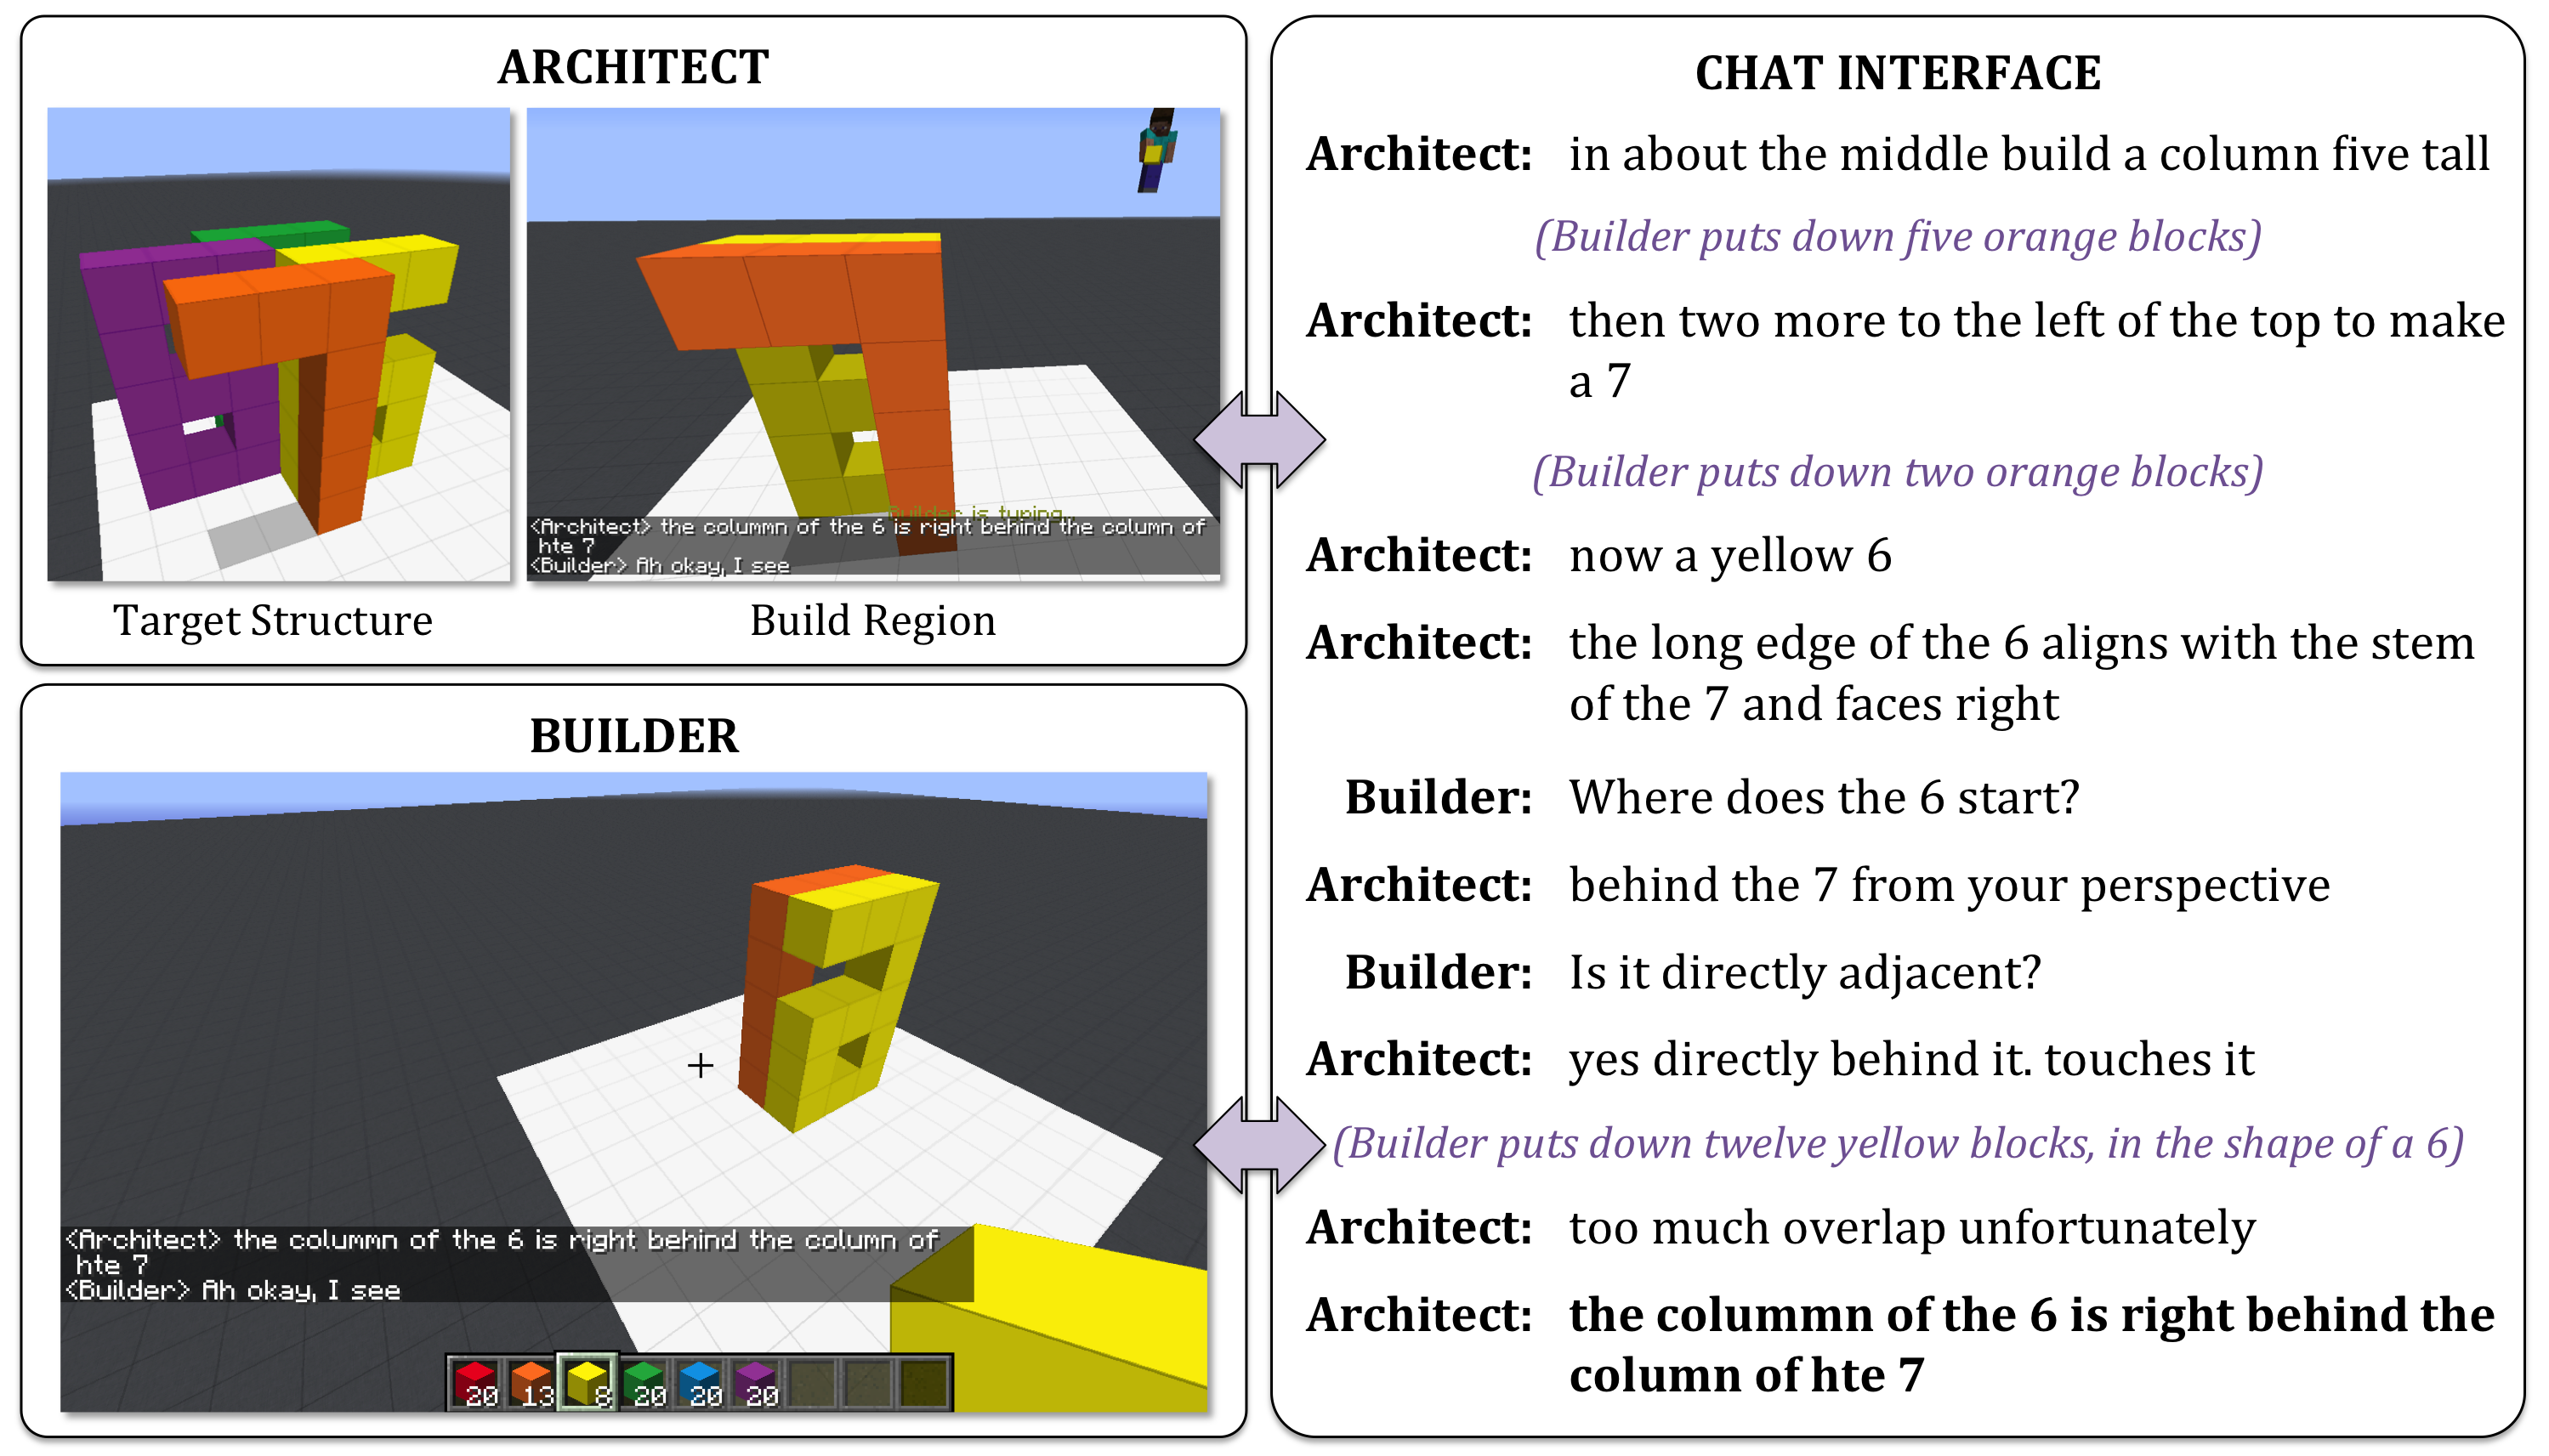
\includegraphics[width=.7\linewidth]{Narayan-ChenEtAl2019.png}};
\only<-3>{\node[fill,white,rectangle,anchor=east,minimum width=.352\linewidth,minimum height=5.55cm] at (image.east) {};}
\only<-2>{\node[fill,white,rectangle,anchor=south west,minimum width=.35\linewidth,minimum height=3cm] at (image.south west) {};}
\node[anchor=north] at (image.south) {\tiny Source:  \citeauthor{Narayan-ChenEtAl2019} \citeyear{Narayan-ChenEtAl2019}};
\end{tikzpicture}}}

\addtocounter{beamerpauses}{3}
\pause
Collection des Dialogues\footnote<.(1)->{Minecraft Dialogue Corpus \raisebox{-.5ex}{
\includegraphics[width=1em]{GitHub-Mark-32px.png}}} \pause\textrightarrow{} Génération d'énontiations\pause\ (Architect est un robot)

\pause
~\\
Et si le Builder était un robot?\pause
\\
\small \citeauthor{JayannavarEtAl2020}~\citeyear{JayannavarEtAl2020} (Pas de raisonnement spatial)
\end{frame}

\begin{frame}{Travail}

  \vfill
  Établir l'architecture pour créer une preuve de concept\pause\ qui associe
  \begin{itemize}
    \item Traitement automatique des langues (NLP)
    \item Overworld
  \end{itemize}


  % \tableofcontents
  \onslide<+(1)->{\tableofcontents[subsectionstyle=hide/hide/hide]}

\end{frame}

\section{Structure}

\subsection{Architecture}
\tikzset{image/.style={inner sep=0cm},rectangle/.style={},<->/.tip={latex[scale=2]}}
\begin{frame}{Architecture}

\centering
\vfill

\resizebox{0.6\linewidth}{!}{
\begin{tikzpicture}[node distance={.1cm and 1cm}]
  % MINECRAFT
  \node[image] (architect) at (-1,0) {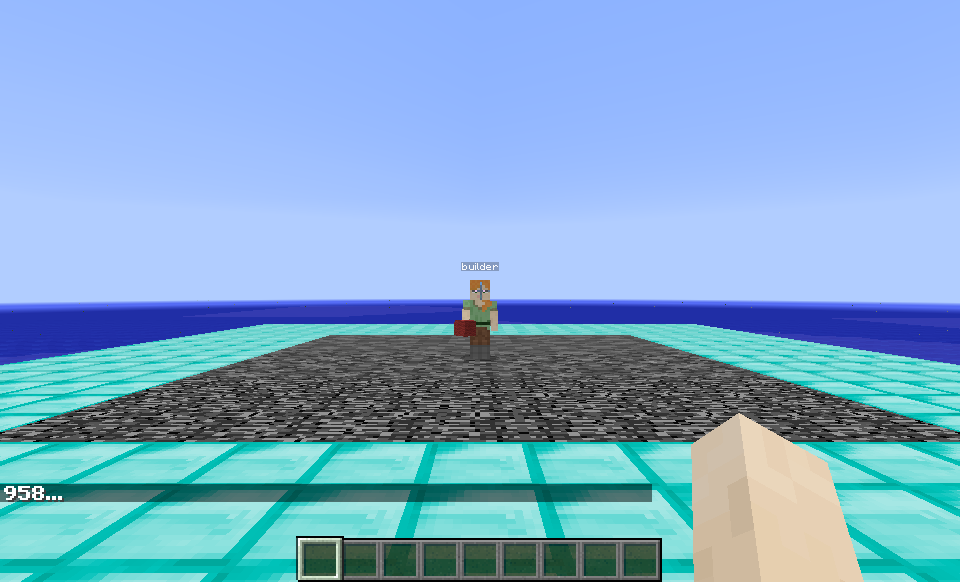
\includegraphics[width=2cm]{architect.png}};
  \node[below=of architect] (architect_text) {\small Architect};
  \node[image,right=of architect] (builder) {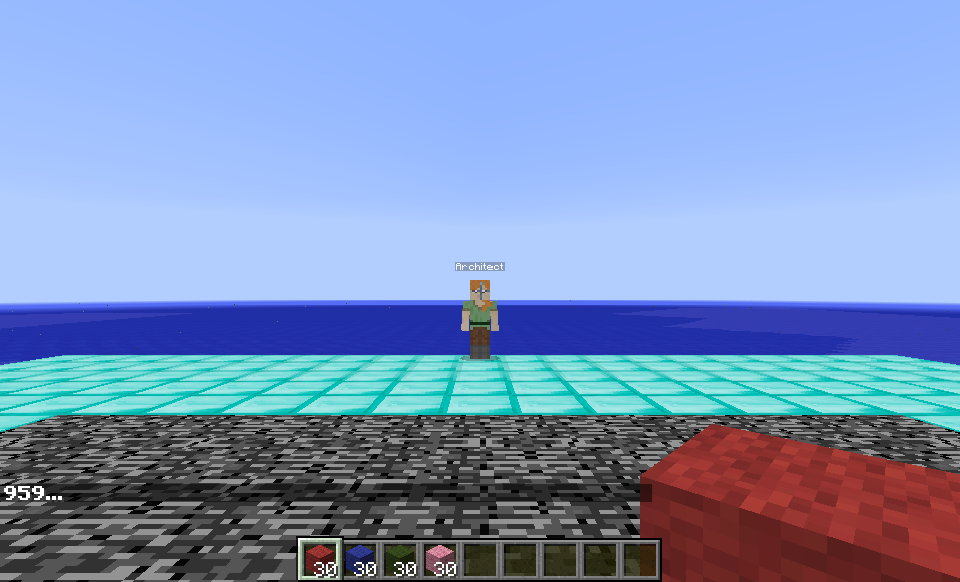
\includegraphics[width=2cm]{builder.png}};
  \node[below=of builder] (builder_text) {\small Builder};
  \onslide<2->{\node[below=of architect_text] (minecraft_text) {\Large Malmö};}
  \node[inner sep=0cm,right=-.1cm of minecraft_text] {
\includegraphics[clip,width=2cm,trim={1cm 30cm 0 25cm}]{minecraft_logo.png}};

  \coordinate (malmodouble) at ($(architect.west |- minecraft_text.south west) + (builder.north east)$);
  \coordinate (malmo) at ($0.5*(malmodouble)$);

  \node[draw,rectangle,minimum width=6.cm,minimum height=3.5cm] (malmo_node) at (malmo) {};


\onslide<3->{
  \node[draw,rectangle,fill=LemonChiffon1,above=4.7cm of malmo,minimum width=5cm,minimum height = 2cm,align=center] (malmo_interface) {\Large Malmö Interface\\ \small nœud ROS};
}
\onslide<2->{
  \draw[<-]  ([xshift=-.5cm]malmo_interface.south-|builder.north) -- ([xshift=-.5cm]builder.north) node[above,sloped,midway] {Stats};
  \draw[->] ([xshift=0cm]malmo_interface.south-|builder.north) -- ([xshift=.0cm]builder.north) node[above,sloped,midway] {Commands};
  \draw[->] ([xshift=.5cm]malmo_interface.south-|builder.north) -- ([xshift=.5cm]builder.north) node[above,sloped,midway] {Chat};

  \draw[<-] ([xshift=.25cm]malmo_interface.south-|architect.north) -- ([xshift=.25cm]architect.north) node[above,sloped,midway] {Chat};
  \draw[<-] ([xshift=-.25cm]malmo_interface.south-|architect.north) -- ([xshift=-.25cm]architect.north) node[above,sloped,midway] {Stats};
}

\onslide<5->{
  \node[draw,rectangle,fill=LightBlue1,above left=2.cm of malmo_interface,minimum width=4cm,minimum height= 2cm,align=center] (dialog_manager) {\Large Dialog Manager\\ \small nœud ROS};
}

\onslide<4->{
  \draw[->] (malmo_interface.190) -| (dialog_manager.250) node[above,sloped,near start] {Chat from Architect};
}
\onslide<6->{
  \draw[<-] (malmo_interface.170) -| (dialog_manager.290) node[above,sloped,near start] {Chat to Builder};
}

\onslide<8->{
  \node[draw,rectangle,fill=Tan1,above right=2.cm of malmo_interface,minimum width=4cm,minimum height= 2cm,align=center] (reasoner) {\Large Planner\\ \small nœud ROS};
}

\onslide<10->{
  \draw[<-] (malmo_interface.10) -| (reasoner.230) node[above,sloped,near start] {Actions};
}
\onslide<9->{
  \draw[->] (malmo_interface.40) |- (reasoner.200) node[above,sloped,near end] {World State};
}
\onslide<7->{
  \draw[->] ([shift={(0cm,.4cm)}]dialog_manager.east) -- ([shift={(0cm,.4cm)}]reasoner.west) node[above,sloped,near end] {Filtered Tasks};}
\onslide<11->{
  \draw[<-] ([shift={(0cm,-0.1cm)}]dialog_manager.east) -- ([shift={(0cm,-0.1cm)}]reasoner.west) node[above,sloped,near end] {Common Errors};}

\end{tikzpicture}
}
\end{frame}

\subsection{Flux de données}

\begin{frame}{Flux de données}

  \vfill
  \begin{itemize}
    \item Malmö API \only<2->{(\texttt{json})}
          \begin{itemize}[<.(2)->]
            \item Stats
            \item Chat
            \item Grid Observations
            \item Commands
          \end{itemize}
    \item ROS
          \begin{itemize}[<.(3)->]
            \item Chat (\texttt{StampedString})
            \item Filtered Tasks (\texttt{StampedString})
            \item Tasks (\texttt{StampedString})
            \item Positions agents/blocs \textrightarrow\ Overworld (\texttt{*Poses})
          \end{itemize}
    \item Ontologenius
          \begin{itemize}[<.(4)->]
            \item Positions des agents/blocs \tikzmark{a}
            \item Couleurs des blocs \tikzmark{ab}
          \end{itemize}
  \end{itemize}
      \onslide<4->{\begin{tikzpicture}[overlay, remember picture,decoration={brace,amplitude=2pt}]
      \draw[decorate,thick] (a.north east) -- (a.north east |- ab.south east) node[midway, right=0.1cm,text=black,text width = 2in] {Inheritance\\ ObjectProperty};
    \end{tikzpicture}
  }

\end{frame}

\subsection{Tâches}
\begin{frame}{Tâches}
  \vfill
  \pause
  ``Put a blue block on your left''

  \vfill
  \begin{description}[<+(1)->]
    \item[Filtered Task] possible tâche complexe (\texttt{PUT(left,blue)})
    \item[Task] Une tâche assez simple (\texttt{TURN(LEFT)}, \texttt{PUT(blue)}, \texttt{TURN(RIGHT)})
    \item[Commands] Action faite par Builder (\texttt{turn}, \texttt{setPitch}, \texttt{place})
  \end{description}
\end{frame}


\section{Tâches réalisées}
\begin{frame}{État}

\begin{itemize}
  \item Stage Ismail (\texttt{.json} + replay)
  \item Docker Image
\end{itemize}
\end{frame}

\section{Petit exemple}

\section{Conclusion}

\begin{frame}{Conclusion}
  \begin{itemize}
    \item<+->
  \end{itemize}
\end{frame}

\begin{frame}[plain]
  \centering
  \vfill
  \begin{minipage}[t]{.5\linewidth}
    \small
    \centering
    Contact\\
% qrencode mailto:rafael.accacio.nogueira@gmail.com?subject=Audition IMT-Atlantique 2024 -o qrContact.png
    \href{mailto:rafael.accacio.nogueira@gmail.com?subject=Audition IMT-Atlantique 2024}{rafael.accacio.nogueira@gmail.com}

    
\includegraphics[width=2cm]{qrContact.png}
  \end{minipage}
  \ifwebcast{\tikz{\draw[fill=pink,draw=pink] (1.5,0) circle [radius=1.5cm]}}%
  \fi
\end{frame}

\appendix

\end{document}
